$server.cpp$ es la implementación del ciclo principal del servidor. Su función es establecer las conexiones con los jugadores y controladores y atenderlos mediante dos funciones:

\begin{itemize}
	\item void atender\_jugador(int i): Dado un mensaje del jugador i, ejecuta el comando pedido y envía la respuesta y los eventos pendientes para este jugador.
	\item void void atender\_controlador(): Dado un mensaje del controlador, ejecuta el comando y envía la respuesta.
\end{itemize}

Mediante la creación de varios threads se buscará:

\begin{itemize}
	\item Permitir que múltiples jugadores puedan conectarse al $backend$ de forma simultánea.
	\item Permitir que uno o varios controladores se conecten al backend en cualquier momento sin importar el estado del juego y puedan obtener los puntajes de los jugadores con el comando Get\_Scores.
\end{itemize}

Para ello realizamos diversas modificaciones en el código del server previsto. Disponemos de un $main$ $thread$ encargado de orquestar todo el sistema distribuyendo trabajos a otros $threads$.

Cuando un jugador quiere conectarse al juego el $main$ $thread$ realiza las siguientes operaciones:

\begin{itemize}
	\item[1] Espera que la conexión sea aceptada por el servidor.
	\item[2] Crea un nuevo $thread$ que atiende al jugador entrante mediante la función $atencion\_p$ (Habrá tantos $threads$ como jugadores haya en el sistema).
	\item[3] El jugador es atendido hasta que finalice el juego.
	\item[4] Cuando finaliza el juego, el $thread$ encargado de atender al jugador termina avisándole al $main$ $thread$.
\end{itemize}

Pseudocódigo:

\begin{algorithmic}
  \Function{Jugador}{}
	\State $pthread\_t \ threads[MAX\_JUGADORES]$ 
	\State $int \ tids[MAX\_JUGADORES]$
	\For{jugador = 0 to n}
		\State accept(jugador)
		\State $pthread\_create(\&threads[i],NULL,atencion\_p,\&tids[jugador])$
	\EndFor
  \EndFunction
\end{algorithmic}

La función encargada de atender a los jugadores es:

\begin{algorithmic}
  \Function{atencion\_p}{jugador}
	\State $bool$ $sale$ $=$ $false$ 
	\While {$!sale$}
		\State atender\_jugador(jugador)
		\State sale = model->termino()
	\EndWhile
	\State $pthread\_exit(NULL)$
  \EndFunction
\end{algorithmic}

Habrá un $thread$, creado por el $main$ $thread$, encargado de atender a los controladores de forma similar a la de los jugadores: aceptando la conexión y creando un nuevo $thread$ por cada controlador.

Una vez que todos los $threads$ encargados de atender a los jugadores y controladores finalizan, el $main$ $thread$ termina su ejecución. Para comprender mejor el accionar del server, presentamos un esquema ilustrativo:


\begin{figure}[H]
\centering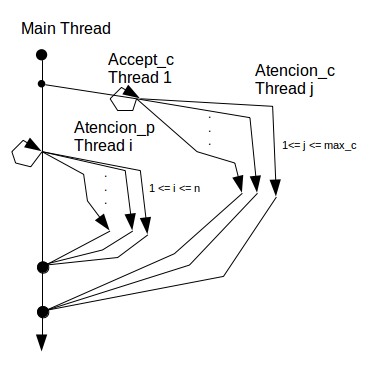
\includegraphics[scale=0.7]{imgs/server.png}
\caption{Esquema del funcionamiento del server.}
\end{figure}

